\section{Simulation of the selected strategies}
\label{sc:simofstrat}
\head{This section contains simulations and verifications of the previously selected formation control strategies separated in steps from initial structure to complete formation control.}
\subsection{The potential field strategy}
The theory of potential fields are implemented with the strategy proposed in section \ref{sc:potential-fields}. The potential field is generated for each individual agent at every update step to make the formation move and converge to a specified formation and position. The field is generated based on forces acting in a overlying potential field structure where one force converges the agent to a desired position, a force attracting the agent to obtain the desired formation along the trajectory, a force repelling the agent from other agents is their distance is too small and finally a force repelling the agents from static objects. The latter two can seem the same, but the repelling force will be larger for the agent-agent force due to the fact that two agents could have course directly toward each other and a more aggressive avoidance can be needed.

To be able to generate and simulate the potential field the implementation needs to be generic. First it was developed with one agent that needs to converge to a desired position and afterwards were other agents added as obstacles and some static objects were added in extend. From these obstacles it can be seen that a single agent are able to converge to a position which makes it possible to expand such that more agents can converge into formation with reference from either a virtual leader or from each other. This will solve the formation coordination task, where the following task will be the group coordination task. The group coordination task has the goal to move the formation around, which here will be done by making the virtual leader, or a actual leader of the formation, follow a trajectory specified. This will make the other agents follow this leader and withhold their formation on the trajectory.
\begin{figure}[htbp]
  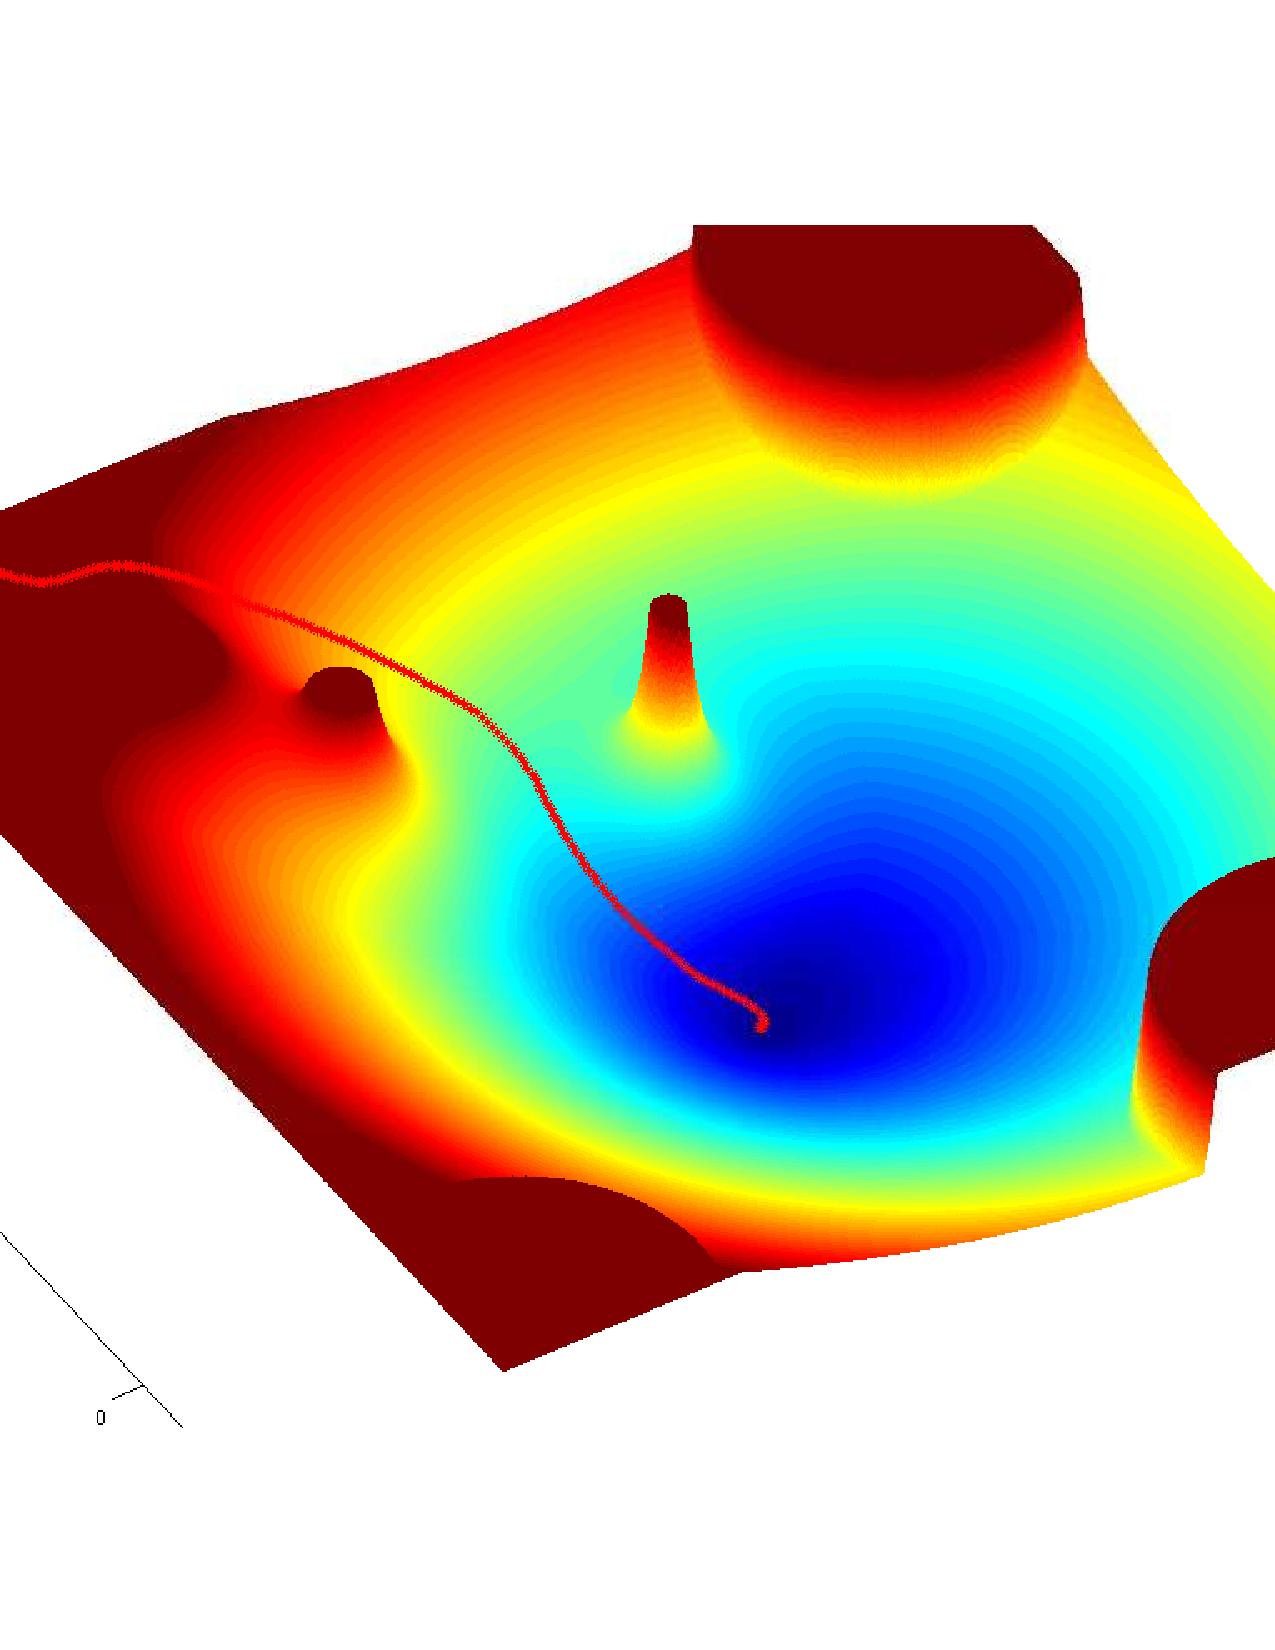
\includegraphics[width=0.9\textwidth]{../../code/matlab/ftotmagnfig1}
  \caption{Plot of one agent's trajectory with the desired position with obstacles to avoid}
  \label{fig:potfieldagenti}
\end{figure}
A plot for a total potential reference field for a single agent can be seen on figure \ref{fig:potfieldagenti}. The red line made of crosses are the trajectory that one single agent will follow, if the obstacles in the plot are static. In the plot every object, either an other agent or an object, are kept static. So it shows how the trajectory will be in one single time step. This will change in the next time step if the other agents also move in the potential field. \todo{Dette er også et mål at få lavet plot af}. \todo{Husk ikke at lave '\\'}.


The grid in which the potential field is generated are limited with a certain resolution while simulating the agents movement. This reduces the directions of where the agents can move, which will not arise a problem on the same level when implemented in reality. In the simulation environment it reduces the resolution such that a single field in the grid contains one value of magnitude of the potential field, which makes the basis of a certain gradient to the field. The agents are following the implementation of the steepest decent. This generates a gradient towards the steepest decent, which makes the agent track this. The analogy can be seen as a bowl, or sphere in this case, where a ball will converge towards the lowest point in the direction of the minimum gradient.

The method of applying the grid with magnitude of the potential field arises the problem with resolution, but also a problem that makes the 'corners' of the grid around the agent to be more likely to have the steepest decent. This problem has been expanded with a solution such that a certain radius around an agent will be checked. The value at the radius around the agent can be checked, and due to the equal distance to every point, these will be weighted equally with respect to their value. This makes the possibility to in principle make the agent go in all directions which will be closer to the reality. When testing the two methods against each other it is clear that the first proposed with the grid structure did not have the same mobility thus not preferable though simpler.

Another problem that can become crucial arises when two objects are within the radius of each other. This will result in a local minima in the potential field between those objects. If an agent converges toward this minima they cannot get out again. The problem can be seen on figure \todo{Lav fig til at vise dette}. Solutions to this problem can be formulated in different ways. One solution could cluster the two objects together and instead of making their potential field individually, then combine those together and make an ellipsoid or even a circle formed obstacle of those objects. This will ensure that the local minima disappears thus not making an agent get stuck between those objects.

In the end this results in that the every agent needs a magnitude and a direction of which they should move. This will be given depending on the total environment where the agents are manoeuvring. When applying this formation strategy a collision free movement are guaranteed which is one of the more critical criteria to be fulfilled. \todo{Det her skal der nok skrives lidt matematik om som viser det, eller en god forklaring. Men dog er det jo en naturlig del af pot field.}
